\documentclass[../main/main.tex]{subfiles}


\begin{document}

\section{March 27th, 2019}
\subsection{Computation of Eigenvalue Decomposition}
For simplicity, we assume that $A\in \R^{n\times n}$ is symmetric, so that all eigenvalues/eigenvectors are real. Let $\lambda_i$ $i=1,2\ldots,n$ be the eigenvalues of $A$, which are sorted in magnitude, i.e.  \[
|\lambda_1|\ge |\lambda_2|\ge \ldots\ge |\lambda_n|
.\] 
The corresponding eigenvectors are denoted by $q_i$. We have  \[
	Q=\begin{bmatrix} q_1 & q_2 &\ldots& q_{n}  \end{bmatrix} \in \R^{n\times n}
\] satisfying $Q^{T}Q=Q^{T}=I$.
\begin{definition}\index{Rayleigh quotient}
	Let $A\in \R^{n\times n}$ be symmetric. For a given vector $x\in \R^{n}$, the \vocab{Rayleigh Quotient} is defined by  \[
		r(x)=\frac{x^{T}Ax}{x^{T}x}
	.\] If $x$ is an eigenvector, \[
	r(x)=\frac{x^{T}Ax}{x^{T}x}= \frac{\lambda x^{T}x}{x^{T}x}=\lambda
,\] i.e. $r(x)$ is an eigenvalue.
\end{definition}
The eigenvalues are critical points of $r(x)$, with $\nabla r(x)=0$. It can be proven that  \[
	\min_i \lambda_i=\min_{x\neq 0} r(x)
.\]
\begin{remark}
	This can be extended to non-symmetric matrices/ matrices or eigenvalues that are complex.
\end{remark}
\subsection{Power Iteration}\index{power iteration}
Purpose: Find $\lambda_1$ and its associated eigenvector $x_1$, with $\|x_1\|_2=1$.
\begin{algo}
	\begin{enumerate}
		\item Choose $y^{(0)}\in R^{n}\text{ s.t. }\|y^{(0)}\|_2=1$.
		\item for $k=1,2,\ldots,n$ \[
				z^{(k)}=Ay^{(k-1)}
		\] \[
		y^{(k)}=\frac{z^{(k)}}{\|z^{(k)}\|_2}
		\] \[
		\mu^{(k)}=\frac{\left( y^{(k)} \right)^{T}Ay^{(k)}}{\left( y^{(k)} \right) ^{T}y^{(k)}}=\left( y^{(k)} \right)^{T}Ay^{(k)}.
	\] 
	\end{enumerate}
\end{algo}
	\begin{remark}
		$y^{(k)}$ is an approximation to $\pm x_1$, $\mu^{(k)}$ is an approximation to $\lambda_1$.
	\end{remark}
\begin{itemize}
	\begin{figure}[htpb]
		\centering
		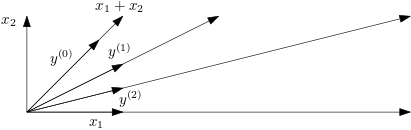
\includegraphics[width=0.6\textwidth]{3-27-power-iteration1.png}
		\caption{}
		\label{fig:}
	\end{figure}
	\item Assume $(2,x_1)$, $(1,x_2)$ are two eigenpairs of $A\in \R^{2\times 2}$ (so that $x_1\perp x_2$). 
	\item Assume $y^{(0)}=\frac{1}{\sqrt{2} }\left( x_1+x_2 \right) $
	\item $k=1$:
		\[
			z^{(1)}=Ay^{(0)}=A\left( \frac{1}{\sqrt{2} }(x_1+x_2) \right) =\frac{1}{\sqrt{2} }(Ax_1+Ax_2)=\frac{1}{\sqrt{2} }(2x_1+x_2)
		.\] \[
		y^{(1)}=\frac{1}{\sqrt{5} }(2x_1+x_2) 
		.\] Note that $y^{(k)}$ approaches $x_1$ more than $x_2$.\\
		$\vdots$
	\item $k+1$ :
		\[
			z^{(k+1)}=Ay^{(k)}=A\left( \frac{1}{\sqrt{2^{2k}+1}}\left( 2^{k}x_1+x_2 \right)  \right)=\frac{1}{\sqrt{2^{2k}+1}}\left( 2^{k+1}x_1+x_2 \right) 
.\] If the component of $x_1$ is non-zero, then it will converge to $x_1$, i.e. as long as $y^{(0)}$ is not a multiple of $x_2$, it will converge to $x_1$.
\end{itemize}
\begin{claim}
	Power iteration may not be convergent:
\end{claim}
\begin{example}
	Assume $(1,x_1)$, $(-1,x_2)$ are two eigenpairs of $A\in \R^{2\times 2}$. Assume $y^{(0)}=\frac{1}{\sqrt{2} }\left( x_1+x_2 \right) $. 
	 \[
		 k=1: z^{(1)}=Ay^{(0)}=\frac{1}{\sqrt{2} }\left( x_1-x_2 \right) 
	.\] \[
	y^{(1)}=\frac{1}{\sqrt{2} }(x_1-x_2)
	.\] \[
	k=2:z^{(2)}=\frac{1}{\sqrt{2} }\left( x_1+x_2 \right) 
	\]\[y^{(2)}=\frac{1}{\sqrt{2} }\left( x_1+x_2 \right) 
	.\] which just repeats itself.
\end{example}

\begin{remark}
	Try with $\left( -2,x_1 \right) $, $(1,x_2)$. Does not converge, but we can get the direction of $x_1$ since both $x_1$ and $-x_1$ are eigenvectors.\\

\end{remark}
\begin{remark}
Power iteration may not converge to $\left( \lambda_1,x_1 \right) $, e.g. $y^{(0)}=x_2$. This is because there is no $x_1$ component.
	
\end{remark}
\subsection{Analysis of Power Iteration}
We will show $|\langle y^{(k)},x\rangle|\to 1$. It is the same as $1-\langle y^{(k)},x_1\rangle^{2}\to 0,\ k\to \infty$
\begin{theorem}
	Assume $A\in \R^{n\times n}$ is symmetric and $|\lambda_1|>|\lambda_2|$ (otherwise they might be amplified at the same rate).\\

	If $\langle y^{(0)}, x_1\rangle \neq 0$, then $\exists  C_0>0$ depending on $y^{(0)}$ only such that  \[
		\left( 1-\langle y^{(k)},x_1\rangle^2 \right) ^{\frac{1}{2}}\le C_0 \left| \frac{\lambda_2}{\lambda_1} \right|^{k}\to 0, \text{ as } k\to \infty 
	.\] Consequently, 
	\begin{itemize}
	\item $\min \{\|y^{(k)}-x_1\|_2,\|y^{(k)}+x_1\|_2\}\le \sqrt{2}C_o \left| \frac{\lambda_2}{\lambda_1} \right| ^{k}$, i.e. $y^{(k)}\to \pm x_1$
		\item $|\mu^{(k)}-\lambda_1|\le 2\sqrt{2} C_o\left| \frac{\lambda_2}{\lambda_1} \right| ^{k}\to 0$
	\end{itemize}
\end{theorem}
\begin{proof}
	Note that \[
		y^{(k)}=\frac{A^{k}y^{(0)}}{\|A^{k}y^{(0)}\|_2}
	.\] 
	Let $A=X\Lambda X^{T}$ be the eigenvalue decomposition of $A$. Then  \[
		A^{k}=X\Lambda X^{T} X\Lambda X^{T}\ldots X\lambda X^{T}=X\Lambda^{k}X^{T}
	.\] So  \[
	A^{k}y^{(0)}=X\Lambda^{k}X^{T}y^{(0)}=X\Lambda^{k}v
	\] \[
	A^{k}y^{(0)}=\begin{bmatrix} x_1&x_2&\ldots&x_n \end{bmatrix}\begin{bmatrix} \lambda_1^{k} v_1\\ \vdots\\ \lambda_n^{k} v_n\end{bmatrix}=\sum_{i=1}^{n} \lambda_i^{k}v_ix_i,\ v_i\in \R,\ x_i\in \R^{n} 
	.\] Because $x_i$ are othronormal,  \[
	\|A^{k}y^{(0)}\|^{2}_2=\sum_{i=1}^{n} \lambda^{2k}_i v^2_1 = \sum_{i=1}^{n} |\lambda_i|^{2k}|v_i|^{2}=|\lambda_1|^{2k}|v_1|^2\left( 1+\ldots \right)\ge \left( |\lambda_1|^{k}|v_1| \right)^2  
	\]  and  \[
	\langle y^{(k)}, x_1\rangle^2=\frac{1}{\|A^ky^{(0)}\|^2_2}\langle A^ky^{(0)},x_1\rangle^2=\frac{1}{\|A^ky^{(0)}\|^2_2}\langle \sum_{i=1}^{n} \lambda_i^{k}v_ix_i,x_1\rangle^2=\frac{1}{\|A^ky^{(0)}\|^2_2}\left( \lambda_1^{k}v_1 \right)^2 
	.\] 
	%\[
	%	1-\langle y^{(k)},x_1\rangle^2=\frac{1}{\|A^{k}y^{(0)}\|^2_2}\left( \|A^k y^{(0)}^2_2\|- |\lambda^k_1 v_1|^2 \right) 
	%.\]
\[
	\le \left| \frac{\lambda_2}{\lambda_1}^{2k} \right| \left( \left| \frac{v_2}{v_1} \right|^2+\left| \frac{v_3}{v_1} \right|^2+\left| \frac{v_4}{v_1} \right|^2+\ldots+ \left| \frac{v_n}{v_1} \right|^2\right) =C_0^2\left| \frac{\lambda_2}{\lambda_1}^{k} \right| 
.\] Thus  \[
\sqrt{1-\langle y^{(k)},x_1\rangle^2}\le C_0\left| \frac{\lambda_2}{\lambda_1}^{k} \right| 
.\] Because $C_0<+\infty$, as $v_1=\angle x_1,y^{(0)}\neq0$ by assumption, \[
\sqrt{1-\langle y^{(k)},x_1\rangle^2}\le C_0\left| \frac{\lambda_2}{\lambda_1}^{k} \right|\to 0, \text{ as } k \to \infty 
.\]\[
\langle y^{(k)},x_1\rangle^2\ge 1-C_0^2\left| \frac{\lambda_2}{\lambda_1}^{2k} \right| \implies \langle y^{(k)},x_1\rangle^2\le \|y^{(k)}\|^2_2\|x_1\|^2_2=1
.\] So \[
1-C_0^2\left| \frac{\lambda_2}{\lambda_1}^{2k} \right| \le 1
.\]  If $\langle y^{(k)},x_1\rangle\ge 0$, then  \[
\|y^{(k)}-x_1\|_2=\sqrt{\|y^{(k)}\|^2_2+\|x_1\|^2_2-2\langle y^{(k)},x_1\rangle}=\sqrt{2-2\langle y^{(k)},x_1\rangle}\le \left( 2-2\sqrt{1-C_0^2\left| \frac{\lambda_2}{\lambda_1}^{2k}  \right|}   \right) ^{\frac{1}{2}}
.\] I give up  will do this later
\end{proof}
\begin{remark}
	\begin{enumerate}
		\item $\langle y^{(k)}, x_1\rangle=\cos \theta$. Genearlly,  \[
				\cos \angle(x,y) = \frac{\langle x,y\rangle}{\|x\|_2\|y\|_2}
		.\] 
	\item The convergenec rate depends on $\left| \frac{\lambda_2}{\lambda_1} \right| <1$, the smaller $\left| \frac{\lambda_2}{\lambda_1} \right| $, the faster the convergence. When $|\lambda_1|=|\lambda_2|$, the power iteration may not converge.
	\item When $\langle y^{(0)},x_1\rangle=0$, then $C_0=+\infty$, so $y$ will not converge to  $\lambda_1$.
	\item In power iteration, only one matrix-product and several vector operations are used, the ocst per step is $O(n^2)$. If we want an approximate eigenvalue/eigenvector of error $\epsilon$, we need to choose $k$, s.t. \[
	C\left| \frac{\lambda_2}{\lambda_1} \right| ^{\frac{k}{2}}\le \epsilon\implies\left| \frac{\lambda_1}{\lambda_2} \right| ^{\frac{k}{2}}\ge \frac{c}{\epsilon}
	.\] \[
	\frac{k}{2}\log\left| \frac{\lambda_1}{\lambda_2} \right| \ge \log\left( \frac{c}{\epsilon} \right) \implies k\ge \frac{\log\left( \frac{c}{\epsilon} \right) }{\log\left( \left| \frac{\lambda_1}{\lambda_2} \right|  \right) }\sim O\left( \log\left( \frac{1}{\epsilon} \right)  \right) 
	.\] Then the total computational cost is \[
	O\left( \log\left( \frac{1}{\epsilon} \right)\cdot n^2 \right)
	.\] 
\item Only the matrix-cector product involving $A $ is needed. This means that $A$ is not needed explicitly, only the subroutine to compute  $Ax$ is sufficient.
	\end{enumerate}
\end{remark}
\end{document}


